\newpage
\begin{center}
    \Huge{\textbf{\underline{Chapter 1: Cryptography}}}
\end{center}

\setcounter{section}{0}

\section{Cryptography}
\begin{prettyBox}{Definition}{myblue}
The word \textbf{cryptography} is derived from two Greek words:
\begin{itemize}
    \item \textbf{Crypt}: means "hidden".
    \item \textbf{Graphy}: means "writing".
\end{itemize}
\end{prettyBox}

\vspace{0.5cm}

\section{Why We Need Cryptography}
\begin{prettyBox}{Need}{myblue}
Cryptography is essential for securing data and communications.
It provides:  
\begin{itemize}
    \item \textbf{Confidentiality}: Ensures that only authorized users can access sensitive information.
    \item \textbf{Data Integrity}: Guarantees that data has not been altered or tampered with during transmission or storage.
    \item \textbf{Availability}: Ensures that authorized users can access data and services when needed.
\end{itemize}
\end{prettyBox}

\vspace{0.5cm}


\section{Some Terminology}

\subsection{Cryptology}
\begin{prettyBox}{Cryptology}{myblue}
Sub filed of math it's the study of secure communication techniques, including both cryptography (creating secure systems) and cryptanalysis (breaking them).
\end{prettyBox}

\vspace{0.25cm}

\subsection{Cryptography}
\begin{prettyBox}{Cryptography}{myblue}
The practice of designing secure communication methods to protect information from unauthorized access.
\end{prettyBox}

\vspace{0.25cm}
\subsection{Cryptanalysis}
\begin{prettyBox}{Cryptanalysis}{myblue}
The study of breaking cryptographic systems to decode encrypted messages without knowing the secret key by finding
the key or part of it , the plain-text or part of it.
\end{prettyBox}

\vspace{0.25cm}
\subsection{Encryption}
\begin{prettyBox}{Encryption}{myblue}
The process of converting plain text into cipher text using an encryption algorithm and a key.
\end{prettyBox}

\vspace{0.25cm}
\subsection{Decryption}
\begin{prettyBox}{Decryption}{myblue}
The process of converting cipher text back into plain text using the correct decryption key.
\end{prettyBox}

\vspace{0.25cm}
\subsection{Cryptographic Algorithm}
\begin{prettyBox}{Cryptographic Algorithm}{myblue}
A mathematical procedure used for encryption and decryption to secure data.
\end{prettyBox}

\vspace{0.25cm}
\subsection{Crypto System}
\begin{prettyBox}{Crypto System}{myblue}
A system that implements cryptographic techniques to secure communications, including encryption algorithms, keys, and protocols.
\end{prettyBox}

\vspace{0.25cm}
\subsection{Plain Text}
\begin{prettyBox}{Plain Text}{myblue}
The original, readable text before encryption.
\end{prettyBox}

\vspace{0.25cm}
\subsection{Cipher Text}
\begin{prettyBox}{Cipher Text}{myblue}
The unreadable, encrypted version of plain text.
\end{prettyBox}

\vspace{0.25cm}
\subsection{Key}
\begin{prettyBox}{Key}{myblue}
A secret value used in cryptographic algorithms to encrypt or decrypt data.
\end{prettyBox}

\vspace{0.25cm}
\subsection{Steganography}
\begin{prettyBox}{Steganography}{myblue}
The practice of hiding information within other non-secret data, such as images, audio files, or text.
\end{prettyBox}


\vspace{1cm}

\section{Categories of Cryptography}

\begin{prettyBox}{Categories}{myblue}
Cryptography can be broadly classified into two major categories:

\begin{itemize}
    \item \textbf{Substitution:} Each letter or group of letters in the
plaintext is replaced with a different letter, number, or symbol.
    \item \textbf{Transposition:} The positions of characters in the plaintext
are rearranged according to a fixed pattern.
\end{itemize}

Additionally, substitution ciphers can be divided into three subcategories:

\begin{itemize}
    \item \textbf{Monoalphabetic:} Maps each plaintext character to one 
ciphertext character. Examples include the Caesar cipher, Shifting cipher,
Affine cipher, and Random substitution.
    \item \textbf{Polyalphabetic:} Maps each plaintext character to multiple
ciphertext characters using different substitution alphabets, making frequency
analysis more difficult. An example is the Vigenère cipher.
    \item \textbf{Polygraphic:} Encrypts groups of letters 
(digraphs, trigraphs, etc.) rather than individual letters. Examples include
the Playfair cipher and Hill cipher.
\end{itemize}
\end{prettyBox}

\vspace{1cm}


\begin{prettyBox}{Reminder}{red}
\textbf{\underline{Modulo Arithmetic}} \\[0.15cm]
In all the upcoming ciphers, modular arithmetic will play a crucial role. We will
frequently use the modulo operation (\textbf{mod}) to keep the index in bound. Here’s how to 
compute \( a \text{ mod } b \):
\begin{itemize}
    \item If \( a = b \), then \( a \text{ mod } b = 0 \).
    \item If \( 0 \leq a < b \), then \( a \text{ mod } b = a \).
    \item If \(a > b\) then \(a \text{ mod } b = a - b\cdot \left\lfloor \dfrac{a}{b} \right\rfloor \)
    \item If \( a < 0 \), then \( a \text{ mod } b = ( -a \text{ mod } b ) + b \).
\end{itemize}
\end{prettyBox}

\section{Classical Cryptography \& Cryptanalysis}
\subsection{Caesar Cipher}

\begin{prettyBox}{Caesar Cipher}{myblue}
The Caesar cipher is a mono-alphabetic substitution cipher used by Julius Caesar, where each letter of the
alphabet is shifted by a fixed amount (commonly 3) to the right. The alphabet is labeled from
0 to 25.

\begin{itemize}
    \item \textbf{Encryption:}  
        \[\boxed{C = E(p,k) = (p + k) \hspace{0.2cm} \text{mod} \hspace{0.2cm} 26}\]
    \item \textbf{Decryption:}  
        \[\boxed{p = D(C,k) = (C - k) \hspace{0.2cm} \text{mod} \hspace{0.2cm} 26}\] 
\end{itemize}

Where:
\begin{itemize}
    \item \(C\) is the ciphered character.
    \item \(p\) is the plain character.
    \item \(E\) is the encryption function.
    \item \(D\) is the decryption function.
    \item \(k\) is the key (shift value).
\end{itemize}
\end{prettyBox}

\vspace{1cm}

\textbf{\underline{Example}}

\begin{center}
    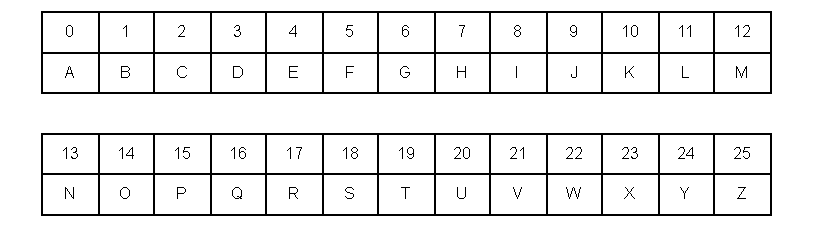
\includegraphics[width=0.8\textwidth]{Chapters/Diagram/Crypto/tab.drawio.pdf}
\end{center}

\vspace{0.5cm}
\textbf{\underline{Encryption Of RABAH}}\\[0.2cm]
\(C_1 = E(17,3) \hspace{0.2cm} \text{mod} \hspace{0.2cm} 26 = 20 \hspace{0.2cm} \text{mod} \hspace{0.2cm} 26 = \boxed{20}\)\\[0.15cm]
\(C_2 = E(0,3) \hspace{0.2cm} \text{mod} \hspace{0.2cm} 26 = 3 \hspace{0.2cm} \text{mod} \hspace{0.2cm} 26 = \boxed{3}\)\\[0.15cm]
\(C_3 = E(1,3) \hspace{0.2cm} \text{mod} \hspace{0.2cm} 26 = 4 \hspace{0.2cm} \text{mod} \hspace{0.2cm} 26 = \boxed{4}\)\\[0.15cm]
\(C_4 = E(0,3) \hspace{0.2cm} \text{mod} \hspace{0.2cm} 26 = 3 \hspace{0.2cm} \text{mod} \hspace{0.2cm} 26 = \boxed{3}\)\\[0.15cm]
\(C_5 = E(7,3) \hspace{0.2cm} \text{mod} \hspace{0.2cm} 26 = 10 \hspace{0.2cm} \text{mod} \hspace{0.2cm} 26 = \boxed{10}\)\\[0.15cm]

\[\text{RABAH} \hspace{0.2cm} \Longrightarrow \hspace{0.2cm} \text{UDEDK} \]

\newpage
\textbf{\underline{Decryption Of ODWHA}}\\[0.2cm]
\(p_1 = D(14,3) \hspace{0.2cm} \text{mod} \hspace{0.2cm} 26 = 11 \hspace{0.2cm} \text{mod} \hspace{0.2cm} 26 = \boxed{11}\)\\[0.15cm]
\(p_2 = D(3,3) \hspace{0.2cm} \text{mod} \hspace{0.2cm} 26 = 0 \hspace{0.2cm} \text{mod} \hspace{0.2cm} 26 = \boxed{0}\)\\[0.15cm]
\(p_3 = D(22,3) \hspace{0.2cm} \text{mod} \hspace{0.2cm} 26 = 19 \hspace{0.2cm} \text{mod} \hspace{0.2cm} 26 = \boxed{19}\)\\[0.15cm]
\(p_4 = D(7,3) \hspace{0.2cm} \text{mod} \hspace{0.2cm} 26 = 4 \hspace{0.2cm} \text{mod} \hspace{0.2cm} 26 = \boxed{4}\)\\[0.15cm]
\(p_5 = D(0,3) \hspace{0.2cm} \text{mod} \hspace{0.2cm} 26 = -3 \hspace{0.2cm} \text{mod} \hspace{0.2cm} 26 = \boxed{23}\)\\[0.15cm]

\[\text{ODWHA} \hspace{0.2cm} \Longrightarrow \hspace{0.2cm} \text{LATEX} \]


\vspace{0.75cm}

\subsection{Shifting Cipher}
\begin{prettyBox}{Shifting Cipher}{myblue}
The shifting cipher is a mono-alphabetic substitution cipher that shifts each
letter of the alphabet left or right by \( k \) positions.
If \( k = 3 \) and the shift is to the right, it becomes 
the Caesar cipher.

\begin{itemize}
    \item \textbf{Encryption:}  
        \begin{center}
        \boxed{C = E(p,k) = (p + k) \hspace{0.2cm}\text{mod} \hspace{0.2cm} 26} \quad \text{(Right shift)}
        
        \vspace{0.15cm}
        \hspace{-0.25cm}\boxed{C = E(p,k) = (p - k) \hspace{0.2cm}\text{mod}\hspace{0.2cm} 26} \quad \text{(Left shift)}   
        \end{center}
            \item \textbf{Decryption:}  
                \[\boxed{p = D(C,k) = (C - k) \hspace{0.2cm} \text{mod} \hspace{0.2cm} 26} \quad \text{(Right shift decryption)}\]  
                \[\hspace{-0.25cm}\boxed{p = D(C,k) = (C + k) \hspace{0.2cm}\text{mod}\hspace{0.2cm} 26} \quad \text{(Left shift decryption)}\]  
\end{itemize}
\end{prettyBox}

\vspace{1cm}

\subsection{Random Substitution}
\begin{prettyBox}{Random Substitution}{myblue}
Random substitution is a type of \textbf{mono-alphabetic substitution cipher} 
where each letter in the plaintext is randomly mapped to a unique ciphertext
letter. The key for this cipher is the mapping table itself, which defines
the substitution for each letter.
\end{prettyBox}

\vspace{1cm}

\textbf{\underline{Example}}

\vspace{0.5cm}

\begin{center}
    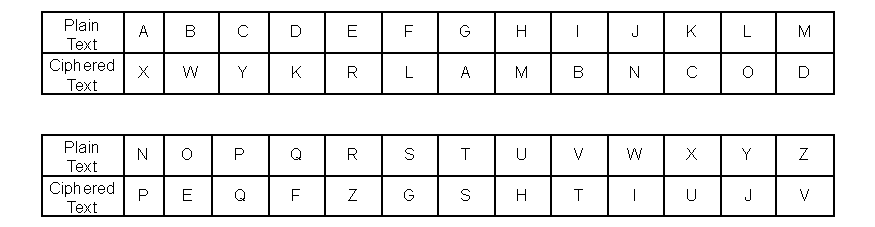
\includegraphics[width=0.8\textwidth]{Chapters/Diagram/Crypto/rc.drawio.pdf}
\end{center}



\subsection{Affine Cipher}
\begin{prettyBox}{Affine Cipher}{myblue}
The affine cipher is a type of monoalphabetic substitution cipher that uses the equation of a line to encrypt and decrypt text.

\begin{itemize}
    \item \textbf{Encryption:}  
        \[\boxed{ E(x, a, b) = (a \cdot x + b) \hspace{0.1cm} \equiv \hspace{0.1cm} y \hspace{0.1cm} [26] }\]
    \item \textbf{Decryption:}  
        \[\boxed{ D(y, a^{-1}, b) = (y - b) \cdot a^{-1}\hspace{0.1cm} \equiv \hspace{0.1cm} x  \hspace{0.1cm} [26] }\]
\end{itemize}

Where:
\begin{itemize}
    \item \(x\) is the plaintext character (represented as an integer in \([0, 25]\)).
    \item \(y\) is the ciphertext character (represented as an integer in \([0, 25]\)).
    \item \(E\) is the encryption function.
    \item \(D\) is the decryption function.
    \item \(b\) is the shift value, \(b \in [0, 25]\).
\item \(a\) is the multiplier, \(a \in [1,26] \) that are coprime with 26.
    \item \(a^{-1}\) is the modular inverse of \(a\) modulo 26.
\end{itemize}
\end{prettyBox}

\vspace{0.65cm}
\begin{prettyBox}{Note}{red}
\begin{itemize}
    \item \textbf{\underline{When \(a = 0\)}}:  
        We lose the original plaintext, and the entire ciphertext will be a sequence of \(b\).  

    \item \textbf{\underline{When \(a = 1\)}}:  
        The affine cipher becomes a Caesar (shift) cipher, shifting each character to the right by \(b\) positions.  
\end{itemize}
\end{prettyBox}

\vspace{1cm}

\subsubsection{How We Found The Decryption Function}
\begin{prettyBox}{Decryption Function}{myblue}
\begin{center}
    \(a \cdot x + b &\equiv y [26]\)\\[0.13cm] 
    \(a \cdot x &\equiv y - b [26]\)\\[0.13cm]
    \(a^{-1} \cdot (a \cdot x) &\equiv a^{-1} \cdot (y - b) [26]\)\\[0.13cm]
    \(x &\equiv a^{-1} \cdot (y - b) [26]\)\\[0.13cm]
  \boxed{\(a^{-1} \cdot (y - b) \equiv x [26]\)}
\end{center}
   
Condition to substitute \(a \cdot a^{-1}\) with 1:
    
\begin{center}
    \(a \cdot a^{-1} &\equiv 1 [26]\)
\end{center}

\end{prettyBox}

\vspace{1cm}

\subsubsection{Why \(a\) Has To Be Coprime With 26}
\begin{prettyBox}{Why \(a\) Has To Be Coprime With 26}{myblue}
\textbf{1. Ciphertext Collisions When \( a \) Is Not Coprime}\\[0.15cm]
If \( a \) is not coprime with 26, multiple plaintext characters can map to the same ciphertext character, making decryption impossible.\\[0.1cm]
Example for \( a = 2 \), \( b = 2 \):

\begin{itemize}
    \item \( x = 0 \):
        \[
            2 \cdot 0 + 2 \equiv y [26] \Rightarrow 2 \equiv y [26] \Rightarrow \boxed{y = 2}
        \]
    \item \( x = 13 \):
        \[
            2 \cdot 13 + 2 \equiv y' [26] \Rightarrow 28 \equiv y' [26] \Rightarrow \boxed{y' = 2}
        \]
\end{itemize}

Here, both \( x = 0 \) and \( x = 13 \) produce the same ciphertext character \( y' = y = 2 \), causing information loss.  
This happens because \( \gcd(2, 26) = 2 \neq 1 \), making decryption impossible.

\vspace{0.75cm}

\textbf{2. Existence of the Modular Inverse}\\[0.15cm]
By definition the modular inverse of \(a^{-1}\) is given with :
\[
    a \cdot a^{-1} \equiv 1 [26]
\]
However, this inverse \textbf{only exists if \( a \) and 26 are coprime}, meaning:
\[
\gcd(a, 26) = 1
\]

\textbf{Proof:} we can prove that From Bézout’s identity :

\begin{center}
    \(a \cdot x + n \cdot k = \gcd(a,n)\)\\[0.13cm]
    \(a \cdot x + 26 \cdot k = \gcd(a,26) = d\)\\[0.13cm] 
    \(a \cdot x = d - 26 \cdot k \)\\[0.13cm]
    \(a \cdot x \equiv d [26]\)\\[0.13cm]
    \(a \cdot a^{-1} \equiv d [26]\)\\[0.13cm]
    \(a \cdot a^{-1} \equiv 1 [26]\)\\[0.13cm]
\end{center}

If \( d = \gcd(a, 26) =  1 \), then \(a^{-1}\) exists by definition only if \(a\) and 26 are coprime. 
\end{prettyBox}

\vspace{1cm}

\subsubsection{Finding \(a^{-1}\)}
\begin{prettyBox}{\(a^{-1}\)}{myblue}
To find \( a^{-1} \), we solve:


\begin{center}
    \(a\cdot a^{-1} \equiv 1 [26]\)\\[0.17cm]
    \(a \cdot a^{-1} = 1 + 26\cdot k\)
\end{center}

which gives:
\[
    \boxed{a^{-1} = \frac{1 + 26\cdot k}{a}}
\]
We try values of \(k\) until \( a^{-1} \) is an integer, which only happens if \( \gcd(a, 26) = 1 \).  
If the result is greater than 26, we reduce it modulo 26 to get \( a^{-1} \) in the range \( [0,25] \).
\end{prettyBox}

\newpage
\textbf{Example With The Key \((a,b) = (5,18)\)}\\[0.15cm]
\textbf{Encryption of SMILE}\\[0.15cm]

\(y_1 = E(18,5,18) \hspace{0.2cm} \text{mod} \hspace{0.2cm} 26 = 108 \hspace{0.2cm} \text{mod} \hspace{0.2cm} 26 = \boxed{4}\)\\[0.15cm]
\(y_2 = E(12,5,18) \hspace{0.2cm} \text{mod} \hspace{0.2cm} 26 = 78 \hspace{0.2cm} \text{mod} \hspace{0.2cm} 26 = \boxed{0}\)\\[0.15cm]
\(y_3 = E(8,5,18) \hspace{0.2cm} \text{mod} \hspace{0.2cm} 26 = 58 \hspace{0.2cm} \text{mod} \hspace{0.2cm} 26 = \boxed{6}\)\\[0.15cm]
\(y_4 = E(11,5,18) \hspace{0.2cm} \text{mod} \hspace{0.2cm} 26 = 73 \hspace{0.2cm} \text{mod} \hspace{0.2cm} 26 = \boxed{21}\)\\[0.15cm]
\(y_5 = E(4,5,18) \hspace{0.2cm} \text{mod} \hspace{0.2cm} 26 = 38 \hspace{0.2cm} \text{mod} \hspace{0.2cm} 26 = \boxed{12}\)\\[0.15cm]


\[\text{SMILE} \hspace{0.2cm} \Longrightarrow \hspace{0.2cm} \text{EAGVM}\]


\vspace{1cm}
\textbf{Decryption of EAGVM}\\[0.15cm]
\textbf{Finding \(a^{-1}\)}\\[0.1cm]
Since \(\gcd(a,26) = \gcd(5,26) = 1\) , \(a^{-1}\) exists :
\begin{center}
    \(a^{-1} = \dfrac{26k+1}{a}\)\\[0.25cm]
    \(a^{-1} = \dfrac{26(4)+1}{5}\)\\[0.25cm]
    \(\boxed{a^{-1} = 21}\)
\end{center}
\vspace{0.75cm}
\(x_1 = D(4,21,18) \hspace{0.2cm} \text{mod} \hspace{0.2cm} 26 = -294 \hspace{0.2cm} \text{mod} \hspace{0.2cm} 26 = \boxed{18}\)\\[0.15cm]
\(x_2 = D(0,21,18) \hspace{0.2cm} \text{mod} \hspace{0.2cm} 26 = -378 \hspace{0.2cm} \text{mod} \hspace{0.2cm} 26 = \boxed{12}\)\\[0.15cm]
\(x_3 = D(6,21,18) \hspace{0.2cm} \text{mod} \hspace{0.2cm} 26 = -252 \hspace{0.2cm} \text{mod} \hspace{0.2cm} 26 = \boxed{8}\)\\[0.15cm]
\(x_4 = D(21,21,18) \hspace{0.2cm} \text{mod} \hspace{0.2cm} 26 = 63 \hspace{0.2cm} \text{mod} \hspace{0.2cm} 26 = \boxed{11}\)\\[0.15cm]
\(x_5 = D(12,21,18) \hspace{0.2cm} \text{mod} \hspace{0.2cm} 26 = -126 \hspace{0.2cm} \text{mod} \hspace{0.2cm} 26 = \boxed{4}\)\\[0.15cm]


\[\text{EAGVM} \hspace{0.2cm} \Longrightarrow \hspace{0.2cm} \text{SMILE}\]

\newpage


\subsection{Hill Cipher With 2x2 Matrix}
\begin{prettyBox}{Hill Cipher}{myblue}
Hill cipher is a polygraphic substitution cipher that uses a square matrix \(n\times n\) ,
it split the text into m vector of n size.

\begin{itemize}
    \item \textbf{Encryption:}  
        \[\boxed{ E(p, K) = K \cdot p \hspace{0.1cm} \equiv \hspace{0.1cm} C \hspace{0.1cm} [26] }\]
    \item \textbf{Decryption:}  
        \[\boxed{ D(C, K^{-1}) = K^{-1} \cdot C \hspace{0.1cm} \equiv \hspace{0.1cm} p  \hspace{0.1cm} [26] }\]
\end{itemize}

\begin{itemize}
    \item \(C\) is the ciphered text.
    \item \(p\) is the plain text.
    \item \(E\) is the encryption function.
    \item \(D\) is the decryption function.
    \item \(K\) is the key the square matrix \(n\times n\) where \(\forall K_{ij} \in [0,25]\). 
    \item \(K^{-1}\) is the inverse matrix.
\end{itemize}

\end{prettyBox}

\vspace{0.65cm}


\subsubsection{Finding \(K^{-1}\)}
\begin{prettyBox}{\(K^{-1}\)}{myblue}
Inverse of any matrix is found using:  
\[
    \boxed{D^{-1} \cdot \operatorname{Adj}(K) \hspace{0.1cm} \equiv \hspace{0.1cm} k^{-1}[26]}
\]

where:  
\begin{itemize}
    \item \(D\) is the determinant of \(K\).
    \item \(\operatorname{Adj}(K)\) is the transpose of the cofactor matrix of \(K\).
\end{itemize}

\vspace{0.4cm}
\textbf{Calculating \(D\) determinant}

\[
K = \begin{pmatrix}
    a & b\\
    c & d
\end{pmatrix}
\Longrightarrow
\boxed{D = ad - bc \text{ mod } 26}
\]

\vspace{0.5cm}

\textbf{Calculating \(D^{-1}\)}\\[0.15cm]
Now that we have \(D\), we need to find \(\dfrac{1}{D}\) or \(D^{-1}\). We need to solve the
same equation as before in affine cipher:

\[
D \cdot D^{-1} \equiv 1 [26]
\]

\[
\boxed{D^{-1} = \frac{26k' + 1 }{D}}
\]

\vspace{0.5cm}
\textbf{Adjoint of \(K\)}\\[0.15cm]
The adjoint of a matrix is the transpose of the cofactor matrix. For a \(2\times2\) matrix:  

\[
\boxed{
\operatorname{Adj} (\begin{pmatrix}
    a & b\\
    c & d
\end{pmatrix}) \text{ mod 26}
= 
\begin{pmatrix}
    d & -b\\
    -c & a
\end{pmatrix}
\text{ mod } 26}
\]
\end{prettyBox}

\newpage

\begin{prettyBox}{Note}{red}
When a given text cannot be divided into \(m\) vectors of size \(n\),  
we need to append extra characters to fill the gap.  
Most of the time, we use 'X' or 'Z'.
\end{prettyBox}

\vspace{1cm}

\textbf{\underline{Example}}\\[0.15cm]
\[K = \begin{pmatrix}
    2 & 3\\
    3 & 6
\end{pmatrix}\]

\textbf{Encryption Of ATTACK}\\[0.15cm]
Divide the word into 3 verctor of size 2
\[
p_1 = \left(\begin{array}{c} A \\ T \end{array}\right) 
= \left(\begin{array}{c} 0 \\ 19 \end{array}\right)
\hspace{0.3cm},\hspace{0.3cm}
p_2 = \left(\begin{array}{c} T \\ A \end{array}\right) 
= \left(\begin{array}{c} 19 \\ 0 \end{array}\right)
\hspace{0.3cm},\hspace{0.3cm}
p_3 = \left(\begin{array}{c} C \\ K \end{array}\right) 
= \left(\begin{array}{c} 2 \\ 10 \end{array}\right)
\]


\[
C_1 = K \cdot p_1 = \begin{pmatrix} 2 & 3 \\ 3 & 6 \end{pmatrix} \cdot \begin{pmatrix} 0 \\ 19
\end{pmatrix} \text{ mod } 26 = \begin{pmatrix} (2 \cdot 0) + (3 \cdot 19) \\ (3 \cdot 0) +
(6 \cdot 19) \end{pmatrix} \text{ mod } 26 = \begin{pmatrix} 57 \\ 114 \end{pmatrix}
\text{ mod } 26 = \boxed{\begin{pmatrix} 5 \\ 10 \end{pmatrix}}
\]

\[
C_2 = K \cdot p_2 = \begin{pmatrix} 2 & 3 \\ 3 & 6 \end{pmatrix} \cdot \begin{pmatrix} 19 \\ 0
\end{pmatrix} \text{ mod } 26 = \begin{pmatrix} (2 \cdot 19) + (3 \cdot 0) \\ (3 \cdot 19) +
(6 \cdot 0) \end{pmatrix} \text{ mod } 26 = \begin{pmatrix} 38 \\ 57 \end{pmatrix}
\text{ mod } 26 = \boxed{\begin{pmatrix} 12 \\ 5 \end{pmatrix}}
\]

\[
C_3 = K \cdot p_3 = \begin{pmatrix} 2 & 3 \\ 3 & 6 \end{pmatrix} \cdot \begin{pmatrix} 2 \\ 10
\end{pmatrix} \text{ mod } 26 = \begin{pmatrix} (2 \cdot 2) + (3 \cdot 10) \\ (3 \cdot 2) +
(6 \cdot 10) \end{pmatrix} \text{ mod } 26 = \begin{pmatrix} 34 \\ 66 \end{pmatrix}
\text{ mod } 26 = \boxed{\begin{pmatrix} 8 \\ 14 \end{pmatrix}}
\]

\vspace{0.5cm}

\[\text{ATTACK} \hspace{0.2cm} \Longrightarrow \hspace{0.2cm} \text{FKMFIO}\]

\vspace{1cm}


\textbf{Encryption Of LATEX}\\[0.15cm]
When dividing LATEX into 3 segments of size 2 ,the last part has a missing element therefore
we will append it with 'X'

\[
p_1 = \left(\begin{array}{c} L \\ A \end{array}\right) 
= \left(\begin{array}{c} 11 \\ 0 \end{array}\right)
\hspace{0.3cm},\hspace{0.3cm}
p_2 = \left(\begin{array}{c} T \\ E \end{array}\right) 
= \left(\begin{array}{c} 19 \\ 4 \end{array}\right)
\hspace{0.3cm},\hspace{0.3cm}
p_3 = \left(\begin{array}{c} X \\ X \end{array}\right) 
= \left(\begin{array}{c} 23 \\ 23 \end{array}\right)
\]


\[
C_1 = K \cdot p_1 = \begin{pmatrix} 2 & 3 \\ 3 & 6 \end{pmatrix} \cdot \begin{pmatrix} 11 \\ 0
\end{pmatrix} \text{ mod } 26 = \begin{pmatrix} (2 \cdot 11) + (3 \cdot 0) \\ (3 \cdot 11) +
(6 \cdot 0) \end{pmatrix} \text{ mod } 26 = \begin{pmatrix} 22 \\ 33 \end{pmatrix}
\text{ mod } 26 = \boxed{\begin{pmatrix} 22 \\ 7 \end{pmatrix}}
\]

\[
C_2 = K \cdot p_2 = \begin{pmatrix} 2 & 3 \\ 3 & 6 \end{pmatrix} \cdot \begin{pmatrix} 19 \\ 4
\end{pmatrix} \text{ mod } 26 = \begin{pmatrix} (2 \cdot 19) + (3 \cdot 4) \\ (3 \cdot 19) +
(6 \cdot 4) \end{pmatrix} \text{ mod } 26 = \begin{pmatrix} 50 \\ 81 \end{pmatrix}
\text{ mod } 26 = \boxed{\begin{pmatrix} 24 \\ 3 \end{pmatrix}}
\]

\[
C_3 = K \cdot p_3 = \begin{pmatrix} 2 & 3 \\ 3 & 6 \end{pmatrix} \cdot \begin{pmatrix} 23 \\ 23
\end{pmatrix} \text{ mod } 26 = \begin{pmatrix} (2 \cdot 23) + (3 \cdot 23) \\ (3 \cdot 23) +
(6 \cdot 23) \end{pmatrix} \text{ mod } 26 = \begin{pmatrix} 115 \\ 207 \end{pmatrix}
\text{ mod } 26 = \boxed{\begin{pmatrix}11 \\ 25 \end{pmatrix}}
\]

\vspace{0.5cm}

\[\text{LATEXX} \hspace{0.2cm} \Longrightarrow \hspace{0.2cm} \text{WHYOLZ}\]

\newpage
\textbf{Decryption Of WHYOLZ}\\[0.15cm]
\textbf{Determinant \(D\)}
\[D = ad - bc \text{ mod } 26 = 2\cdot 6 - 3\cdot 3 \text{ mod } 26 =\boxed{3}\]

\textbf{Finding \(D^{-1}\)}

\[ D\cdot D^{-1} \hspace{0.1cm} \equiv \hspace{0.1cm} 1 [26]\]

\vspace{0.15cm}

\begin{center}
\(D^{-1}  = \dfrac{26k' + 1 }{D}\)\\[0.3cm]
\(D^{-1}  = \dfrac{26(1) + 1 }{D}\)\\[0.3cm]
\(\boxed{D^{-1} = 9}\)
\end{center}

\vspace{0.2cm}
\textbf{Adj(\(K\))}
\[
\operatorname{Adj}( \begin{pmatrix}
    2 & 3\\
    3 & 6
\end{pmatrix}
) \text{ mod } 26
= 
\begin{pmatrix}
    6 & -3\\
    -3 & 2
\end{pmatrix}
\text { mod } 26
= 
\boxed{ \begin{pmatrix}
        6 & 23\\
        23 & 2
\end{pmatrix} }
\]


\textbf{Finding \(K^{-1}\)}\\[0.1cm]
\[K^{-1} = D^{-1} \cdot \text{Adj}(K) \text{ mod } 26 = 9 \cdot \begin{pmatrix}
    6 & 23\\
    23 & 2
    \end{pmatrix} \text{ mod } 26 =  \begin{pmatrix}
    54 & 207\\
    207 & 18
\end{pmatrix} \text{ mod } 26 = \boxed {
\begin{pmatrix}
    2 & 25\\
    25 & 18
\end{pmatrix}
}\]

\vspace{0.5cm}
Dividing the ciphered text into 3 vector of size 2 :

\[
C_1 = \left(\begin{array}{c} W \\ H \end{array}\right) 
= \left(\begin{array}{c} 22 \\ 7 \end{array}\right)
\hspace{0.3cm},\hspace{0.3cm}
C_2 = \left(\begin{array}{c} Y \\ O \end{array}\right) 
= \left(\begin{array}{c} 24 \\ 3 \end{array}\right)
\hspace{0.3cm},\hspace{0.3cm}
C_3 = \left(\begin{array}{c} L \\ Z \end{array}\right) 
= \left(\begin{array}{c} 11 \\ 25 \end{array}\right)
\]

\[
p_1 = K^{-1} \cdot C_1 = \begin{pmatrix} 2 & 25 \\ 25 & 18 \end{pmatrix} \cdot \begin{pmatrix} 22 \\ 7
\end{pmatrix} \text{ mod } 26 = \begin{pmatrix} (2 \cdot 22) + (25 \cdot 7) \\ (25 \cdot 22) +
(18 \cdot 7) \end{pmatrix} \text{ mod } 26 = \begin{pmatrix} 219 \\ 676 \end{pmatrix}
\text{ mod } 26 = \boxed{\begin{pmatrix} 11 \\ 0 \end{pmatrix}}
\]

\[
p_2 = K^{-1} \cdot C_2 = \begin{pmatrix} 2 & 25 \\ 25 & 18 \end{pmatrix} \cdot \begin{pmatrix} 24 \\ 3
\end{pmatrix} \text{ mod } 26 = \begin{pmatrix} (2 \cdot 24) + (25 \cdot 3) \\ (25 \cdot 24) +
(18 \cdot 3) \end{pmatrix} \text{ mod } 26 = \begin{pmatrix} 123 \\ 654 \end{pmatrix}
\text{ mod } 26 = \boxed{\begin{pmatrix} 19 \\ 4 \end{pmatrix}}
\]

\[
p_3 = K \cdot C_3 = \begin{pmatrix} 2 & 25 \\ 25 & 18 \end{pmatrix} \cdot \begin{pmatrix} 11 \\ 25
\end{pmatrix} \text{ mod } 26 = \begin{pmatrix} (2 \cdot 11) + (25 \cdot 25) \\ (25 \cdot 11) +
(18 \cdot 25) \end{pmatrix} \text{ mod } 26 = \begin{pmatrix} 647 \\ 725 \end{pmatrix}
\text{ mod } 26 = \boxed{\begin{pmatrix}23 \\ 23 \end{pmatrix}}
\]


\[\text{WHYOLZ} \hspace{0.2cm} \Longrightarrow \hspace{0.2cm} \text{LATEXX}\]


\vspace{1cm}


\subsection{Playfair Cipher}
\begin{prettyBox}{Playfair Cipher}{myblue}
The Playfair cipher is a polygraphic substitution cipher that encrypts two characters at a time using a \(5 \times 5\) matrix key.

\begin{itemize}
    \item Each cell in the matrix must contain a unique letter.
    \item Since the matrix holds only 25 letters, the letter 'J' is usually omitted.
    \item If the plaintext contains 'J', it is replaced with 'I'.
    \item The key consists of a unique-lettered word placed at the beginning of the matrix.
    \item The remaining cells are filled with the rest of the alphabet in order, excluding any letters already used in the key.
\end{itemize}
\end{prettyBox}

\newpage
\textbf{\underline{Example With Key MONARCHY}}

\begin{center}
    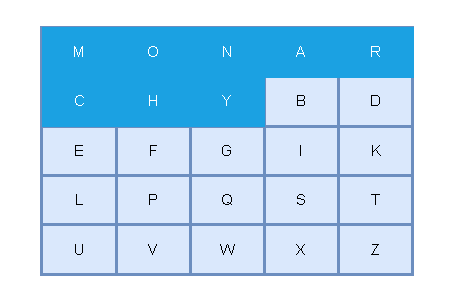
\includegraphics[width=0.6\textwidth]{Chapters/Diagram/Crypto/playfair.drawio.pdf}
\end{center}

\vspace{1cm}


\subsubsection{Splitting Text into Pairs}
\begin{prettyBox}{Splitting}{myblue}
\begin{itemize}
    \item If the number of characters is odd, the text is appended
with the letter 'Z'.
    \item A pair cannot consist of the same letter, in such cases a filler
letter 'X' is inserted between them.
\end{itemize}
\end{prettyBox}

\vspace{0.85cm}
\textbf{\underline{Example}}\\[0.4cm]
INSTRUMENTS \(\Longrightarrow\) IN , ST , RU , ME , NT , TZ\\[0.25cm]
We appended the letter 'Z' because it has an odd number of letters.

\vspace{0.5cm}
HELLO \(\Longrightarrow\) HE , LX , LO\\[0.25cm]
We added the letter 'X' between LL to avoid having pair with same letter.

\vspace{1cm}


\subsubsection{Encryption}

\begin{prettyBox}{Encryption}{myblue}
\begin{itemize}
    \item \textbf{When the pair is in the same column:} Replace each letter
with the one directly below it (wrapping to the top if at the bottom).
    \item \textbf{When the pair is in the same row:} Replace each letter with
the one to its right (wrapping to the leftmost if at the rightmost).
    \item \textbf{Otherwise:} Form a rectangle with the pair and replace each
letter with the one in its opposite horizontal corner.
\end{itemize}
\end{prettyBox}

\newpage

\textbf{\underline{Example Encryption Of INSTRUMENTSZ}}

\vspace{0.5cm}


\begin{center}
    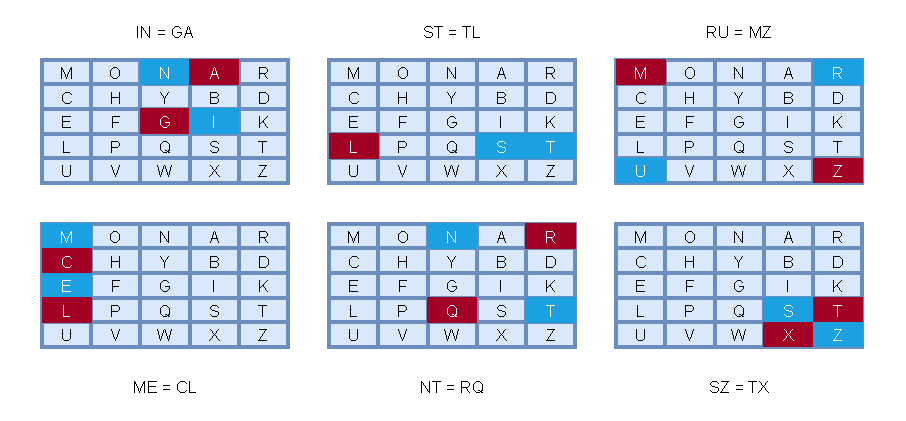
\includegraphics{Chapters/Diagram/Crypto/pf1.drawio.pdf}
\end{center}


\[\text{INSTRUMENTSZ} \hspace{0.2cm} \Longrightarrow \hspace{0.2cm} \text{GATLMZCLRQTX}\]

\vspace{1cm}

\subsubsection{Decryption}
\begin{prettyBox}{Decryption}{myblue}
\begin{itemize}
    \item \textbf{When the pair is in the same column:} Replace each letter
with the one directly above it (wrapping to the bottom if at the top).
    \item \textbf{When the pair is in the same row:} Replace each letter with
the one to its left (wrapping to the rightmost if at the leftmost).
    \item \textbf{Otherwise:} Form a rectangle with the pair and replace each
letter with the one in its opposite horizontal corner.
\end{itemize}
\end{prettyBox}

\vspace{0.85cm}


\textbf{\underline{Example Decryption Of GATLMZCLRQTX}}

\vspace{0.5cm}


\begin{center}
    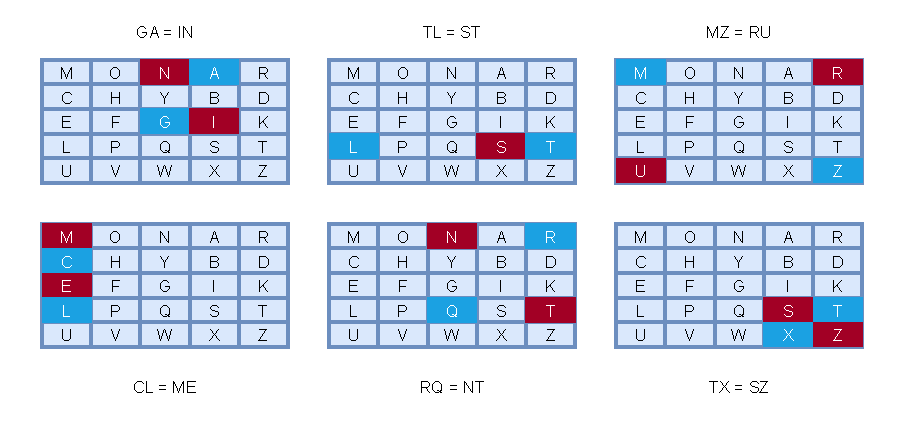
\includegraphics{Chapters/Diagram/Crypto/pf2.drawio.pdf}
\end{center}


\[\text{GATLMZCLRQTX} \hspace{0.2cm} \Longrightarrow \hspace{0.2cm} \text{INSTRUMENTSZ}\]

\newpage

\subsection{Vigenère Cipher}

\begin{prettyBox}{Vigenère Cipher}{myblue}
The Vigenère cipher is a polyalphabetic substitution cipher that uses a repeating key string.

\begin{itemize}
    \item \textbf{Encryption:}  
        \[
        \boxed{C = E(p, k) = (p + k) \hspace{0.2cm} \text{mod} \hspace{0.2cm} 26}
        \]
    \item \textbf{Decryption:}  
        \[
        \boxed{p = D(C, k) = (C - k) \hspace{0.2cm} \text{mod} \hspace{0.2cm} 26}
        \] 
\end{itemize}

Where:
\begin{itemize}
    \item \( C \) is the encrypted character.
    \item \( p \) is the plaintext character.
    \item \( E \) is the encryption function.
    \item \( D \) is the decryption function.
    \item \( k \) is a character from the key string.
\end{itemize}

\end{prettyBox}

\vspace{1cm}

\textbf{\underline{Example With The Key MAP}}\\[0.15cm]
\textbf{\underline{Encryption Of HELLO}}

\vspace{0.25cm}

\begin{center}
    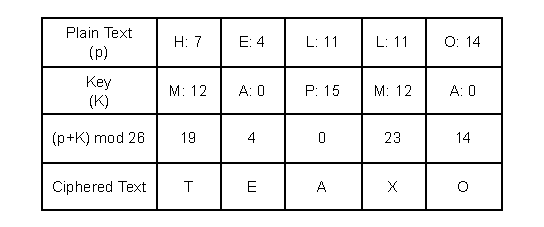
\includegraphics{Chapters/Diagram/Crypto/v1.drawio.pdf}
\end{center}

\vspace{1cm}

\textbf{\underline{Decryption Of TEAXO}}

\vspace{0.25cm}

\begin{center}
    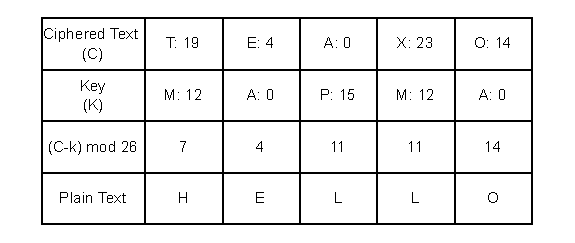
\includegraphics{Chapters/Diagram/Crypto/v2.drawio.pdf}
\end{center}

\newpage

\begin{prettyBox}{Note}{red}
\textbf{\underline{Euler's Totient Function:}}\\[0.15cm]
Euler's Totient Function, denoted \(\phi(n)\), counts the number of integers up to \(n\) that are coprime to \(n\). For a positive integer \(n\) with the prime factorization:
\[
n = \prod_{i=1}^{m} p_i^{\alpha_i}
\]
where \(p_i\) are the distinct prime factors of \(n\) and \(\alpha_i\) are their respective exponents, the totient function is given by:
\[
\phi(n) = n \times \prod_{i=1}^{m} \left(1 - \frac{1}{p_i}\right)
\]
\vspace{0.25cm}

\textbf{\underline{Extended Euclidean Algorithm:}}\\[0.15cm]
The Extended Euclidean Algorithm is used to find the multiplicative inverse of \(a\) modulo \(b\) ,
we first perform the normal Euclidean Algorithm till remainer = 1 then with substitution of the remainers from the bottom we express 1 
as a linear combination of \(a\) and \(b\):
   \[
   1 = a \cdot x + b \cdot y
   \]
The coefficient \(x\) is the multiplicative inverse of \(a\) modulo \(b\)\\[0.1cm]
If \(x < 0\) use modulo to get the final result. 
\end{prettyBox}

\vspace{0.75cm}


\textbf{\underline{Example}}\\[0.15cm]

Find the number of integers coprime to 12:  
\[
12 = 2^2 \times 3^1
\]
\[
\phi(12) = 12 \times \left(1 - \frac{1}{2}\right) \times \left(1 - \frac{1}{3}\right) = \boxed{4}
\]

\vspace{0.25cm}

Find the multiplicative inverse of \(5\) modulo \(12\):  

Using the extended Euclidean algorithm:  
\begin{center}
    \(12 = 5 \times 2 + 2\)\\[0.1cm]
    \(5 = 2 \times 2 + \boxed{1}\)\\[0.1cm]
\end{center}

Back-substituting to express \(1\) as a linear combination of \(5\) and \(12\):  
\[
1 = 5 - 2 \times 2
\]
Since \(2 = 12 - 5 \times 2\), we substitute:  
\[
1 = 5 - (2 \times (12 - 5 \times 2))
\]
\[
1 = 5 - (2 \times 12 - 5 \times 4)
\]
\[
1 = 5 + (-2) \times 12 + 5 \times 4
\]
\[
1 = 5 \times \boxed{5} + 12 \times (-2)
\]

Thus, the modular inverse of \(5\) modulo \(12\) is \(\boxed{5}\).

\newpage

\subsection{Classical Cryptanalysis}  

\begin{prettyBox}{Cryptanalysis}{myblue}  
\begin{itemize}  
    \item \textbf{Brute Force:} A method that systematically tries all possible keys until  
          the correct one is found. It is particularly effective against monoalphabetic  
          ciphers with a small keyspace, such as the Affine cipher (where \( a \) must be  
          coprime with 26).  
    \item \textbf{Frequency Analysis:} A technique that examines the frequency of letters  
          or groups of letters in a given language. Pioneered by Al-Kindi, it is highly  
          effective against monoalphabetic and polygraphic ciphers, as these ciphers tend  
          to preserve the plaintext’s frequency distribution.  
    \item \textbf{Kasiski Test:} A method for breaking the Vigenère cipher, a polyalphabetic  
          cipher. It identifies repeated substrings in the ciphertext, assuming that structured  
          languages cause the key to repeat at regular intervals. By analyzing the distances  
          between these repetitions, one can determine the key length using common factors.  
\end{itemize}  
\end{prettyBox}  

